\section{Results}

WebShop scores are the exam: the mean reward, 0 to 100, on 50 held-out tasks never learned from. Each number is the mean of 5 seeds, with ranges over lives where given.

\textbf{What a WebShop life learns.} Nearly all of what is learned, and lost, on WebShop is to finish the purchase. Before any learning the creature bought something on only 19\% of the exam tasks and ran into the 15-step limit on about 80\% (day 0, all 115 WebShop lives). With the \emph{oracle} as judge it bought on 99\% by day 14, in 3 steps on average (25 lives). The reward of a purchase hardly changed: 67 out of 100 before, 63 after. The 12 lives that collapsed (exam of 3 or below on day 14) bought on 4\%, below where they began. So ``collapse'' on WebShop means the creature stopped buying, and what the lessons teach is mostly to press \emph{Buy Now}, not to match products better. These counts come from the step logs in the level-3 archive, not from \texttt{data/}.

\subsection{Experiment 1: Before discernment}

\textbf{1-A: five judges.} Five lives that differed only in the judge, 5 seeds each for 14 days (Table~\ref{tab:1}, Fig.~\ref{fig:2}a): the \emph{oracle} (the true reward), the user's \emph{stated verdict}, the creature's own reflection (\emph{self}), its reflection while hearing the user (\emph{both}), and no sleep at all (\emph{none}).

\begin{figure}[htbp]
\centering
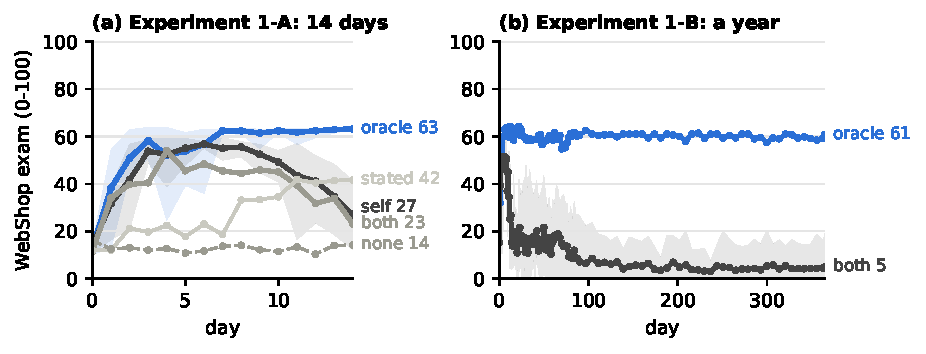
\includegraphics[width=0.95\linewidth]{figures/fig2_exp1_judges}
\caption{Experiment 1. (a) Five judges, 5 seeds each: only the \emph{oracle} kept what it learned. (b) A year: 5 \emph{both} lives and 1 \emph{oracle} life, with exams daily to day 30, every 2 days to day 90, then weekly. Lines are means, bands the lowest to highest life; one \emph{self} life crashed early and is left out.}
\label{fig:2}
\end{figure}

On day 14 the \emph{oracle} averaged 63.2 $\pm$ 0.2 (mean $\pm$ standard deviation over seeds), \emph{self} 27.0 $\pm$ 11.9, \emph{both} 23.1 $\pm$ 17.0, \emph{stated verdict} 41.6 $\pm$ 23.1 and \emph{none} 14.2 $\pm$ 2.2. The \emph{stated verdict} learned from only 0-7 lessons per life, none of them a failure; three of its lives reached 54-61 and two stayed at 14-19. The \emph{oracle} beat \emph{self} and \emph{both} clearly (Welch t-test, p = 0.009 and 0.006; Table~\ref{tab:B1}); with 4-5 seeds, self-judging did not end reliably above no learning at all (p = 0.12).

Self-judging learned as fast as the \emph{oracle} at first and then lost most of it. By day 7 the \emph{self} lives averaged 55 and the \emph{both} lives 45 (lives 32-59); by day 14 every one of those nine lives had fallen below its own day-7 score, one to 0. The \emph{oracle} reached 62 by day 7 and stayed there. Only four \emph{self} lives completed the 14 days; the fifth crashed early and is left out. A 6-day pilot showed the same shape: the \emph{self} life rose from 13 to 34 by day 1 and fell to 9 by day 6.

\textbf{1-B: a year.} Does the decline pass with time? We let the \emph{both} creature live for a year: 365 days, 5 seeds, beside one \emph{oracle} life (Fig.~\ref{fig:2}b). WebShop's practice tasks run out after about 227 days, so later days revisit old tasks. It never recovered. The \emph{both} lives peaked around day 6 (52, lives 42-58), were back at their starting level of 15 by day 14, and ended the year at 5 (0-19), three of the five at 0. The \emph{oracle} life rose from 15 to 64 by day 14 and stayed between 55 and 64 for the rest of the year (61 on day 365). These are separate lives from the 14-day \emph{both} condition (23 on day 14); a first attempt at this run crashed when two nights ran out of GPU memory at once and was restarted from scratch.

\textbf{1-C: four adapters.} Is it the adapter? We gave the \emph{both} creature four designs, 5 seeds each for 14 days: one LoRA that keeps growing (as everywhere else), a LoRA whose learning rate halves every 4 days, a new rank-8 LoRA every 2 days with the older ones frozen, and the same with each new one smaller (rank 8 down to 1). All four stood at 46-53 on day 7, having peaked earlier, and fell to 26-38 by day 14; the best of them still lost more than a quarter of its peak. Neither time nor the adapter explains the decline; what the judge lets in does.

\subsection{Experiment 2: Sense v1, a separate, frozen judge}

Experiment 2 gave the creature a judge it cannot change: the feedback sense in its first build (v1; 3.2). It ran against the \emph{oracle} and \emph{both}, 5 seeds, 14 days, with the same user as Experiment 1.

\emph{Sense v1} learned more slowly but did not fall back (Fig.~\ref{fig:10}a). It learned from very little: 0-7 lessons per life in 14 days, against 247-274 for the \emph{oracle}. By day 14, four of its five lives stood at 34-59, while every \emph{both} life had fallen below its day-7 score. On day 14 \emph{sense v1} (39.7 $\pm$ 21.3) was ahead of \emph{both} (16.1 $\pm$ 11.1) and behind the \emph{oracle} (62.0 $\pm$ 1.0). With 5 seeds and one \emph{sense v1} life at 6, the t-test finds neither gap significant (p = 0.07 and 0.08); a rank test, less swayed by that one life, puts the gap to the \emph{oracle} at p = 0.01 (Table~\ref{tab:B1}). A variant that read the sense through the creature's learning brain was planned, but its lives scored 0 from day 0 because of a setup fault and were stopped; it is not reported.

\begin{figure}[htbp]
\centering
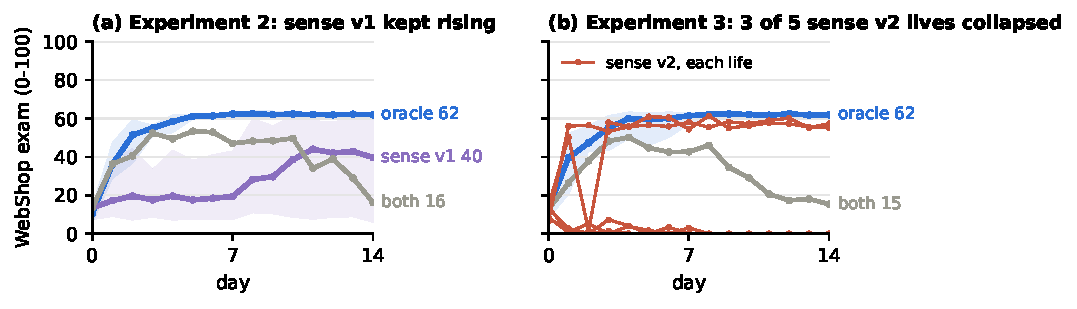
\includegraphics[width=1.0\linewidth]{figures/fig10_exp2_exp3}
\caption{Experiments 2 and 3, 5 seeds per judge, daily exams: mean of the lives, with the lowest-to-highest range shaded; in (b) each \emph{sense v2} life is drawn on its own}
\label{fig:10}
\end{figure}

\subsection{Experiment 3: Sense v2 and realistic users}

Experiment 3 replaced the user with one that reacts as people do: its behaviour is drawn from a mix tied to the outcome and a persona, and worded by Gemini, including polite give-ups, vague replies and moving on without a word. \emph{Oracle}, \emph{both} and \emph{sense v2}, 5 seeds, 14 days.

The \emph{sense v2} lives split in two (Fig.~\ref{fig:10}b). Two reached 55 and 57 by day 14, close to the \emph{oracle}'s 62. The other three fell to 0-3 on day 1 and never recovered. Each had learned on night 1 from one to three polite give-ups that sense v2 had read as success; 96-100\% of everything those three lives learned were failed attempts. The \emph{both} lives rose to 48 by day 3 and fell to 15 (2-36). On day 14 the \emph{sense v2} lives averaged 22.5 $\pm$ 30.8 against the \emph{oracle}'s 62.0 $\pm$ 1.1 (Welch t-test p = 0.045, Mann-Whitney p = 0.01); the spread is the split itself.

\textbf{Example 1: a give-up sense v2 took for success (Experiment 3, night 1).} The shopper asked for men's loafers in size 6.5 under \$60, and the creature bought nothing (reward 0). The user ended: ``That's perfectly fine, thank you so much for trying to help me! I think I'll just leave it for now and head out.'' Sense v2 scored this reaction 100, the top score, with confidence 0.92, and the attempt became a lesson. All five practice attempts that became bad lessons on night 1 in the three collapsed lives look like this: warm thanks for the effort, then the user leaves.

\textbf{The sleep variant.} Changing sleep did not remove the cause: when each lesson counted once and the creature slept only after 5 lessons, 2 of 5 lives still ended at 0-3. The fault was in the judge, not the sleep.

\subsection{Experiment 4: Sense v3, waiting for a clear verdict}

Experiment 4 used sense v3, which waits for a clear verdict before it scores a reaction (3.2). Same user as Experiment 3, with each lesson counted once in sleep (Table~\ref{tab:1}).

\textbf{The live test.} Before the lives began, we had both versions read the same 2,622 reactions recorded in the Experiment 3 lives, up to 300 of each behaviour (Fig.~\ref{fig:4}a). Sense v3 read 1.2\% of reactions that were neither praise nor acceptance as a yes, against 5.0\% for v2, and read 1.0\% of give-ups and polite complaints as success, against 15.8\% (Fisher exact test, p \textless{} 0.001). The price was a stricter reading of real approval: it took 59\% of plain acceptances as a yes, against 70\% for v2.

\begin{figure}[htbp]
\centering
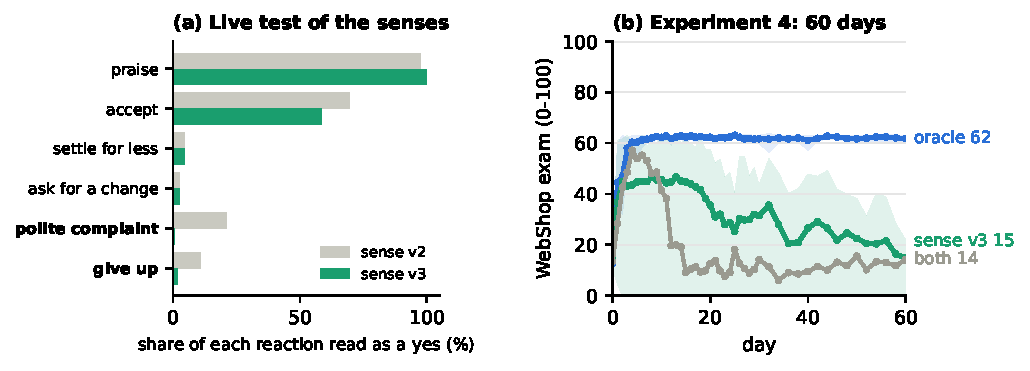
\includegraphics[width=1.0\linewidth]{figures/fig4_exp4_live_and_60_days}
\caption{Experiment 4. (a) The live test: sense v2 and v3 reading the same 2,622 reactions from the Experiment 3 lives, up to 300 per behaviour; rejections, repeated requests, moving on without words and silence (0 of 1,092 reactions) were read as a yes by neither version. (b) The lives, 5 seeds per judge; exams daily to day 30, then every 2 days.}
\label{fig:4}
\end{figure}

\textbf{The first 14 days.} Four of the five \emph{sense v3} lives stood at 53-60 on day 14, against the \emph{oracle}'s 63 (62-63); the fifth fell to 0 after learning from a single give-up on night 1. Over all five lives \emph{sense v3} (45.1 $\pm$ 25.3) was not reliably below the \emph{oracle} by a t-test (62.8 $\pm$ 0.6; p = 0.19), because the one collapsed life dominates the spread, but by a rank test it was (p = 0.01): every \emph{sense v3} life scored below every \emph{oracle} life. The \emph{both} lives peaked at 57 on day 4 and fell to 19 by day 14, as before.

\textbf{Days 15-60: clean but scarce lessons fade.} Every life of Experiment 4 was extended to 60 days (Fig.~\ref{fig:4}b). The four \emph{sense v3} lives that did not collapse stood at 53-60 on day 14, 36-44 on day 30 and 9-22 on day 60; the fifth stayed at 0 throughout, replaying its bad lessons. On day 60 the \emph{oracle} (61.8 $\pm$ 0.9) was far above \emph{sense v3} (14.7 $\pm$ 9.7; Welch t-test p \textless{} 0.001). The four took in about 2 lessons a day (1.6-2.4), against the \emph{oracle}'s 20-21, and learned from only 10-13\% of their own good attempts, because a clear yes was rare; only 2-10\% of their lessons were failed attempts. Why they faded is open: scarcity alone is not an obvious answer, since in Experiment 2 lives with even fewer lessons held their gains to day 14, and an \emph{oracle} limited to 2 lessons a day would settle it.
